This section describes the visual and motor features used in our framework. We begin with the visual features 
(Section \ref{sec:vis-feat}) and then continue with the motor features (Section \ref{sec:mot-feat}).

\subsubsection{Visual Features}
\label{sec:vis-feat}

% \begin{figure}
% 	\centering
% 	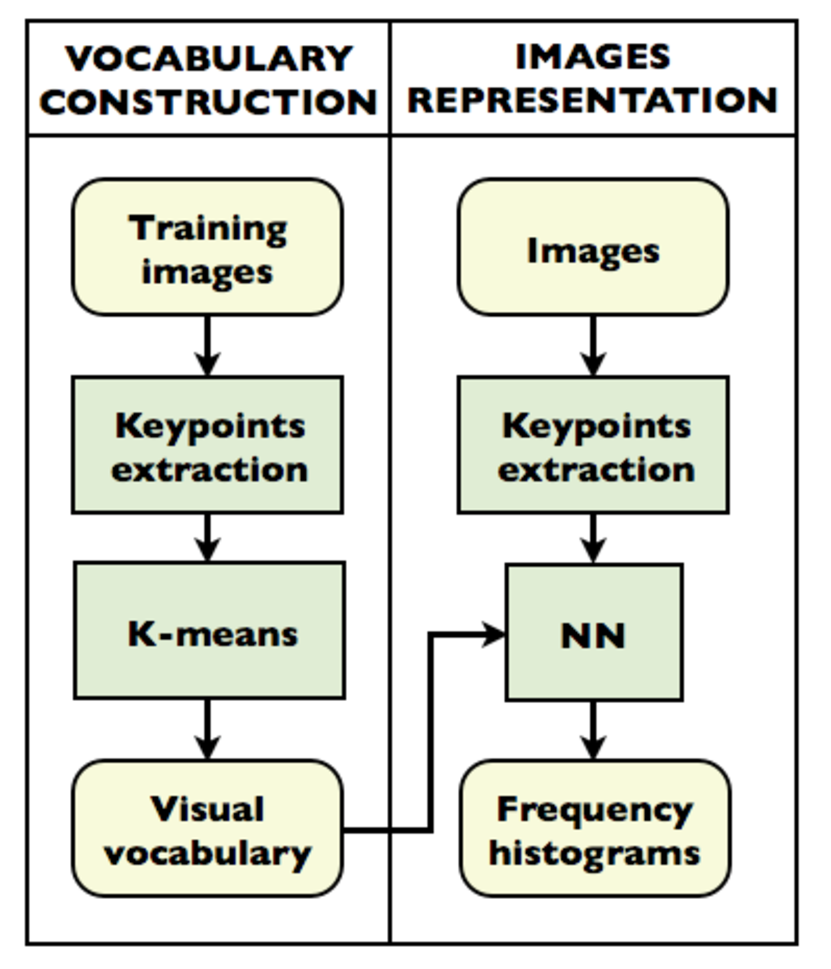
\includegraphics[width=0.5\textwidth]{images/objects/SchemaVisionUnit.pdf}
% 	\caption{A schematic representation of how the visual features are extracted during training(left) and test(right).}
% 	\label{fig::vision}
% \end{figure}

The visual appearance of objects is captured by a dedicated item of the framework, %(see Figure \ref{fig::vision}), 
which
can be sketched as follows.
We first select from the video sequence a set of interesting frames where the object is clearly visible. 
To avoid contamination due to background elements, 
we apply change detection by comparing the selected frames against a background model, and then
restrict our attention on the region of interest (ROI) defined by the object bounding box.
We apply to the ROI a bag-of-keypoints object description \cite{csurka-dance-2004} designed as a two steps procedure \cite{ICIAP}:

\begin{itemize}

\item  We build the global vocabulary, by putting together keypoints extracted from images of all 
the objects into the dataset. As keypoints, we consider a set of randomly sampled points whose 
patch is modeled with a vector valued  descriptor which can be seen as a fixed scale SIFT  \cite{lowe}.
K-means is adopted to cluster the descriptors: the centroids 
(or virtual features) become the words of the visual vocabulary.

\item Both training and test images are thus represented with respect to the vocabulary, with a simple 
nearest neighbor approach.  At the end, visual appearance of objects is summarized with a frequency 
histogram, whose peaks should indicate which virtual features are the most important in modelling a specific object.

\end{itemize}

Notice that the vocabulary size is a system parameter which should be tuned with respect to the complexity of 
objects, to find a trade-off between sparsity of the descriptions and capability of characterizing the objects.           

Finally a remark is in order. From the point of view of appearance-based object recognition, %from visual cues
the experimental scenario is not challenging.
We opted for such a setting in order to keep the focus of the work on the joint modelling of visual and motor inputs.
% being the focus of the work instead to give 
%evidence of the fact that motion actually improves the recognition (classification) performances.

\subsubsection{Motor Features}
\label{sec:mot-feat}
The MPR are simply the $22$ angles returned by the dataglove, considered at
the time of contact of the subject's hand with the object\footnote{A
force-sensing resistor was used to determine the instant of contact.}. The
MPR is therefore a ``snapshot'' of the subject's hand in the instant of
grasping the object.


%\begin{figure}
%	\centering
%	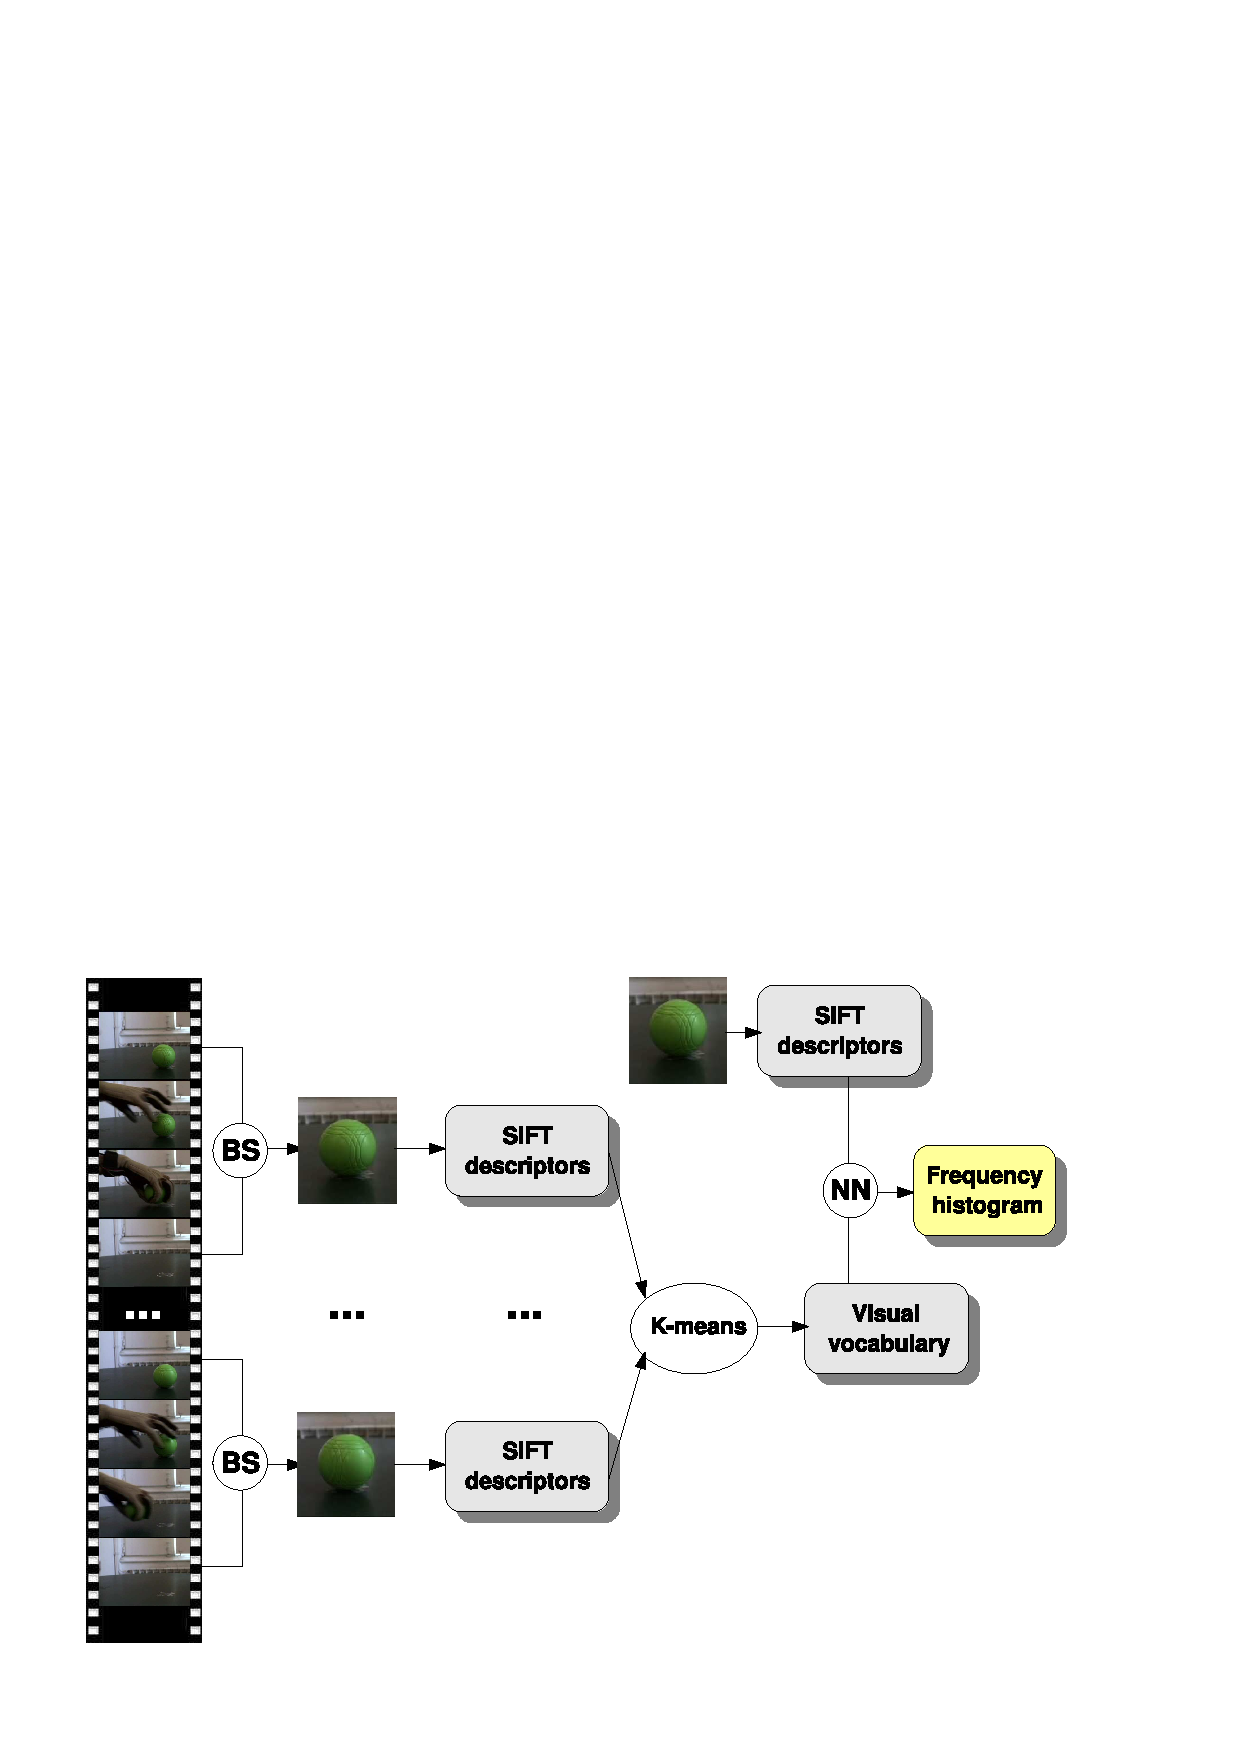
\includegraphics[width=0.5\textwidth]{images/schema_vision.pdf}
%	\caption{A schema of the vision unit. First, suitable frames are extracted from the sequence and objects are located by means of background subtaction (BS). SIFT descriptors of a set of random points are input of a clustering step to get to the final visual vocabulary. Finally, each image is represented with respect to the vocabulary adopting a nearest neighbour (NN) strategy (see text for details).}
%	\label{fig::vision}
%\end{figure}

%As we will discuss in Sec. \ref{sec::experiments}, the system gathers, as one input, a video sequence acting as {\it spectator}, whose focus is on object appearance. The goal of the vision unit is to process the signal to obtain a global model of a set of given objects.
%Figure \ref{fig::vision} shows the pipeline of the vision unit when considering only one object (the same procedure is applied to the whole set of objects). Among the sequence, we first select the frames showing only the object  without any occlusion, then we locate more precisely its position by means of a simple background subtraction. 
%Although in our application there is not an explicit object recognition step, it is clear from the architecture pipeline that a robust and specific object model is functional to subsequent analysis. It is worthwhile also to mention that with the terms {\it object recognition} we indicate the characterization of a specific object instance (againts the concept of categorizing classes of objects).
%We adopt an approach based on local features to describe image structures: because of their popularity a rich variety of local measurements have been proposed in the literature \cite{harris,schmid,lowe} and applied successfully to objects recognition and categorization problems (see \cite{csurka,ferrari} just to name a few). 
%Local approaches tipically include two distinct steps: keypoints extraction and description. 
%However, in our case, a keypoint based-representation often ends up into a poor description
%due to the limited size of the images. We thus built our representation by extracting enough 
%random points  guaranteeing a more homogenous sampling.
%We chose to adopt SIFT descriptors \cite{lowe,schmid2} to model image patches around these points, obtaining a set of {\it words} for each image.\\
%To avoid redundancy and include some global information in our model, we apply k-means \cite{wong}, following the well-known bag-of-words approach \cite{csurka}. 
%We thus build a {\it global} vocabulary, containing SIFT descriptions of all known objects. 
%Image representation is obtained by means of frequency histogram of visual words, selecting for each random point extracted from the image 
%the most similar visual word as nearest neighbor. A normalization step may be advisable for the subsequent data processing.

%\textbf{Questa sezione non mi e' molto chiara....ma la perceptual representation non e'
%fatta da VPR e MPR? Perche' qui descriviamo solo la vision? 
%FEATURES
%---------
%-vision: SIFT, bag of words. 50 words vocabulary, image divided in 4 parts.
%Resulting in feature vectors with 200 elements. 
%-motor: The CyberGlove returns 22 8-bit numbers linearly related to the angles 
%of the subject's hand joints. Resulting in feature vectors with 22 elements.}
